\begin{frame}{Kwantowa strategia}
W kwantowej strategii uzyskamy prawdopodobieństwo wygranej \(\approx 0.85 > 0.75\).\\
Strategia zakłada, że Alicja i Bartosz dzielą dwukubitowy splątany stan
\[\ket{\Psi}=\frac{\ket{00}+\ket{{11}}}{\sqrt{2}}=\frac{1}{\sqrt{2}}\begin{pmatrix}
    1 \\0 \\0 \\1
\end{pmatrix}\]
 Alicji dajemy pierwszy kubit, Bartoszowi drugi.\\
 W zależności od wejścia dokonają innego pomiaru na swoim kubicie
\end{frame}


% ===================================================================


\begin{frame}{}
    Alicja robi pomiar w bazie \(\ket{\alpha}\), \(\ket{\alpha^\perp}\)
    \vspace{-0.7em}
    \[\ket{\alpha}=\cos \theta_A \ket{0} + \sin \theta_A \ket{1}  \qquad \ket{\alpha^\perp}=-\sin \theta_A \ket{0} + \cos \theta_A \ket{1} \]
    Analogicznie Bob robi pomiar w bazie \(\ket{\beta}\), \(\ket{\beta^\perp}\).
    \vspace{-0.7em}
    \[\ket{\beta}=\cos \theta_B \ket{0} + \sin \theta_B \ket{1}  \qquad \ket{\beta^\perp}=-\sin \theta_B \ket{0} + \cos \theta_B \ket{1} \]
    Zatem
    \vspace{-3em}
    \begin{align*}
\sqrt{P(a=0, b=0)}=\braket{\alpha \otimes \beta | \Psi}
&=\frac{1}{\sqrt{2}}
\begin{pmatrix}
\cos \theta_A \cos \theta_B \\
\cos \theta_A \sin \theta_B \\
\sin \theta_A \cos \theta_B \\
\sin \theta_A \sin \theta_B
\end{pmatrix}^T \cdot
\begin{pmatrix}
1 \\
0 \\
0 \\
1
\end{pmatrix}
\\&=\frac{1}{\sqrt{2}}(\cos \theta_A \cos \theta_B+\sin \theta_A \sin \theta_B)=
\\&=\frac{1}{\sqrt{2}}(\cos(\theta_A-\theta_B))
\end{align*}
\end{frame}


% ===================================================================


\begin{frame}{}
    Analogicznie
    \vspace{-3em}
    \begin{align*}
        \sqrt{P(a=1, b=1)}=\braket{\alpha^\perp \otimes \beta^\perp | \Psi}
        &=\frac{1}{\sqrt{2}}
        \begin{pmatrix}
        \sin \theta_A \sin \theta_B \\
        -\sin \theta_A \cos \theta_B \\
        -\cos \theta_A \sin \theta_B \\
        \cos \theta_A \cos \theta_B
        \end{pmatrix}^T \cdot
        \begin{pmatrix}
        1 \\
        0 \\
        0 \\
        1
        \end{pmatrix}
        \\
        &=\frac{1}{\sqrt{2}}(\sin \theta_A \sin \theta_B+\cos \theta_A \cos \theta_B)
        \\
        &=\frac{1}{\sqrt{2}}\cos(\theta_A-\theta_B)
\end{align*}
Więc
\[P(a=b)=\cos^2(\theta_A-\theta_B)\]
\[P(a\neq b)=\sin^2(\theta_A-\theta_B)\]
\end{frame}


% ===================================================================


\begin{frame}{Czego potrzebujemy?}
    Warunek wygranej: \(x\cdot y = a +b \mod{2}\)
    \begin{table}
    \centering
    \begin{tabular}{c|cccc}
    \textbf{Wejście} & $(0,0)$ & $(0,1)$ & $(1,0)$ & $(1,1)$ \\
    \hline
    \textbf{Potrzebujemy} & $a = b$ & $a = b$ & $a = b$ & $a \neq b$
    \end{tabular}
    \end{table}
    \pause
    Dobieramy więc odpowiednio kąty:
    \vspace{0.5em}
     \begin{columns}
     \begin{column}{0.4\textwidth}
    \vspace{-1em}
     \begin{fact}{Strategia Alicji}
        \[ \theta_A=\begin{cases}
             0 \quad \text{dla } x=0\\
              \pi/4 \quad \text{dla } x=1\\
         \end{cases}\]
     \end{fact}
     \end{column}
    \begin{column}{0.4\textwidth}
        \vspace{-1em}

    \begin{fact}{Strategia Bartka}
        \[ \theta_B=\begin{cases}
             \pi/8 \quad \text{dla } x=0\\
              -\pi/8 \quad \text{dla } x=1\\
         \end{cases}\]
     \end{fact}
     \end{column}
 \end{columns}
 Dobraliśmy kąty tak, że \(|\theta_A-\theta_B|=\begin{cases}\pi/8 \text{ gdy chcemy \(a=b\) } \\ 3\pi/8 \text{ gdy chcemy \(a \neq b\)}\end{cases}\)
\end{frame}


% ===================================================================


\begin{frame}{Wynik}
\begin{columns}
\begin{column}{0.65\textwidth}
 Dobraliśmy kąty tak, że 
 \[
 |\theta_A-\theta_B|=
 \begin{cases}
 \pi/8 & \text{gdy chcemy } a=b \\
 3\pi/8 & \text{gdy chcemy } a \neq b
 \end{cases}
 \]
 \[
 P(a=b)=\cos^2(\theta_A-\theta_B), \quad
 P(a\neq b)=\sin^2(\theta_A-\theta_B)
 \]
 \pause
 Zatem prawdopodobieństwo wygranej to:
 \[P_{\text{win}}=\cos^2(\pi/8)=\sin^2(3\pi/8)\approx 0.854\]
\onslide<2>{
Poprzez ograniczenie Tirelsona, można pokazać ze jest to wartość optymalna.
}
\end{column}
\begin{column}{0.35\textwidth}
\centering
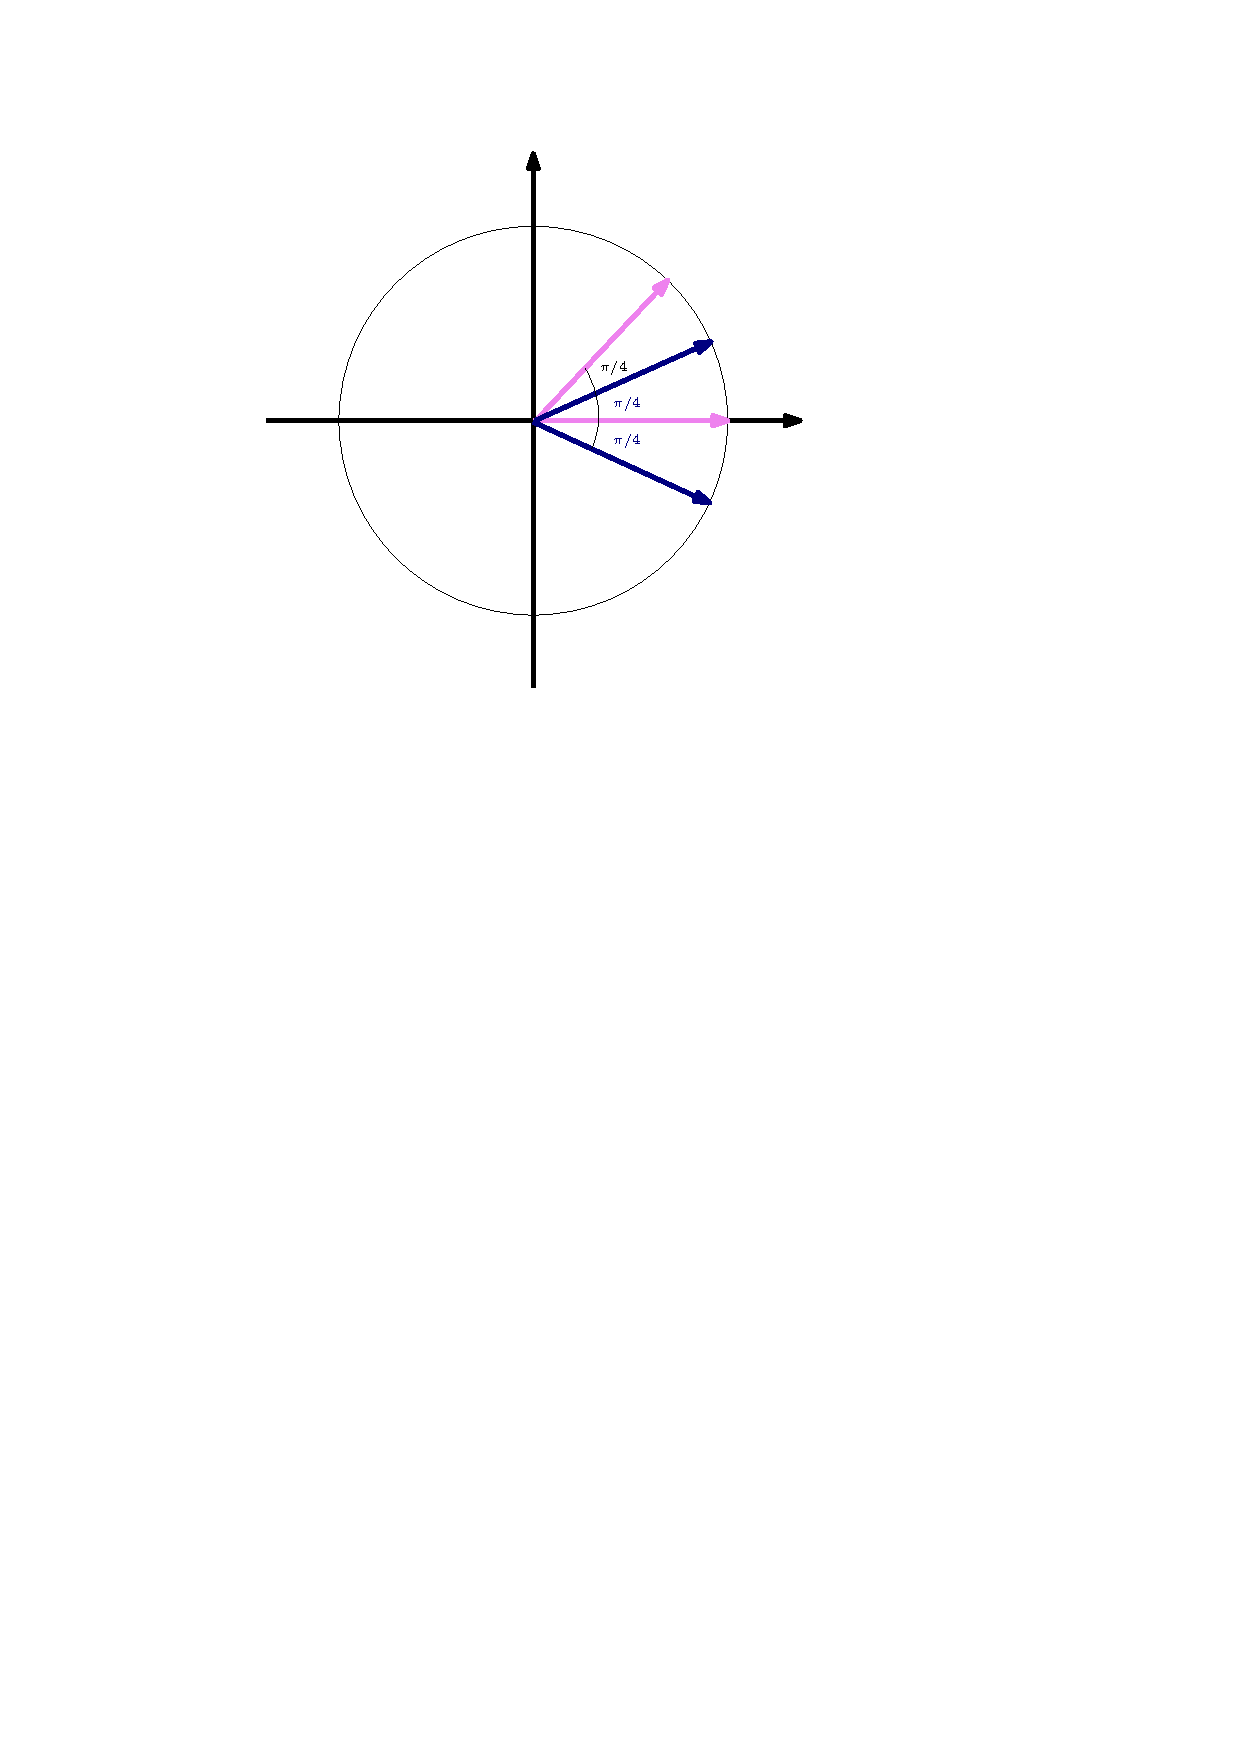
\includegraphics[width=\linewidth]{images/vectors.pdf}

\end{column}
\end{columns}


\end{frame}
\begin{frame}{Uwaga}
    \begin{figure}
        \centering
        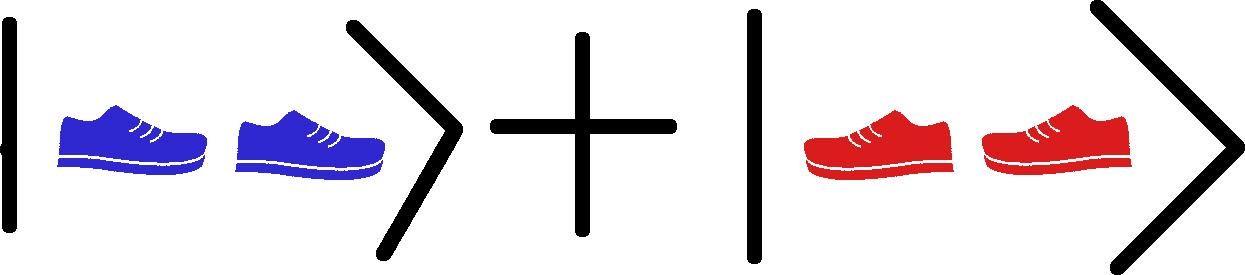
\includegraphics[width=0.5\linewidth]{images/buty.png}
        \label{fig:enter-label}
    \end{figure}
        Istotne jest, że gracze mierzą inne cechy układu (mierzą w innych bazach). Właśnie to daje nam przewagę kwantową.

\end{frame}
\begin{frame}{Związek z nierównością CHSH}
 
Gra CHSH jest równoważna nierówności CHSH. Prawdopodobieństwo wygranej wyraża się wzorem:
\[
  P_{\text{win}} = \frac{S + 4}{8}, \qquad S = 8P_{\text{win}} - 4
\]
gdzie $S = |E(a,b) + E(a,b') + E(a',b) - E(a',b')|$.
 
\medskip
 
\begin{block}{Porównanie granic}
\vspace{-1em}
\begin{center}
\begin{tabular}{lcc}
\toprule
& \textbf{Nierówność CHSH} & \textbf{Gra CHSH} \\
\midrule
Klasyczne & $S \leq 2$ & $P_{\text{win}} \leq \tfrac{3}{4}$ \\[4pt]
Kwantowe (Tsirelson) & $S \leq 2\sqrt{2}$ & $P_{\text{win}} \leq \cos^2\!\tfrac{\pi}{8} \approx 0.854$ \\
\bottomrule
\end{tabular}
\end{center}
\end{block}
 
 
\end{frame}